\documentclass[12pt,a4paper,oneside]{book}

\usepackage[utf8]{inputenc}
\usepackage[english]{babel}
\usepackage{amssymb}
\usepackage{enumitem}
\usepackage{fancyhdr}
\usepackage{setspace}
\usepackage{eurosym}
\usepackage{graphicx}

\fancypagestyle{plain}{
	\fancyhf{}
	\fancyfoot[C]{\thepage}
	\renewcommand{\headrulewidth}{\ifnum\value{chapter}>0 0.5pt \else 0pt \fi}
	\renewcommand{\footrulewidth}{0pt}
	\fancyhead[L]{\ifnum\value{chapter}>0 \bfseries \itshape \nouppercase \leftmark \fi}
}

\pagestyle{plain}

%\onehalfspacing

\newcommand\itemtext[2]{
	\expandafter\gdef\csname item#1\endcsname{#2}
	\label{#1}#2}

\newcommand\refitemtext[1]{\csname item#1\endcsname}

\begin{document}

\tableofcontents

\chapter{Introduction}

\section{Purpose}
The Requirement Analysis and Specifications Document aims to provide in detail every aspect of the service PowerEnJoy, including its components, goals, constraints, functional and non-functional requirements. Use cases and scenarios for all the users involved will be provided as well to conform the product's objectives to the real world.

The last part of this document is reserved to the formalization of some features of the system involving the utilization of Alloy, a declarative specification language which provides a structural modeling tool based on first-order logic.

The high-level functionalities described in the RASD are intended for both developers and project managers. The former have to implement and test the functionalities while the latter must examine whether every requirement has been respected. It may also be useful to users in order to best take advantage of the service.

\section{Description of the problem}
The product described in this RASD is PowerEnJoy, a car-sharing service which offers to its users exclusively electric cars. It includes the common functionalities of its category: permitting to registered users to obtain the position of all the available cars, reserving one within a certain amount of time and continuously displaying the up-to-the-minute cost of the ride are just few of them. Moreover, PowerEnJoy stimulates users to behave virtuously towards the ecosystem by applying various types of discounts under specific conditions.

There are four software components that constitute the PowerEnJoy project. First, a back-end server provides APIs in order to simplify the communication related to the interactions of a user with the cars. Then two applications are available for a user to allow him/her the employment of every functionality: a web-based application (intended for visualization from desktop) and a mobile one. Lastly, every vehicle will be equipped with an on-board computer, used by the driver to manage the ride with the available options and see real-time information related to it, such as the time spent, the distance traveled and the total amount.

\section{Goals}
\begin{enumerate}[label={[G\arabic*]},labelindent=\parindent,leftmargin=*]
	\item \label{goal:registration} Registration of a user to the system
	\item \label{goal:cars_location} Finding the locations of the available cars
	\item \label{goal:reservation} Reservation of a car
	\item \label{goal:expiration} Expiration of reservation and penalization
	\item \label{goal:entry} Entry of registered user into the car
	\item \label{goal:charging} Start charging and notifying the registered user
	\item \label{goal:car_locking} Stop charging the registered user and lock the car
	\item \label{goal:safe_areas} Safe areas for parking the reserved cars
	\item \label{goal:passengers} Detection of extra passengers and applying discount
	\item \label{goal:battery} Detection of the battery status and applying discount
	\item \label{goal:special_areas} Detection of special parking areas and applying discount
	\item \label{goal:constraints} Checking parking and battery constraints and penalization
\end{enumerate}

\section{Domain properties}
\begin{itemize}
	\item User's data are always valid
	\item Location reported by the GPS is always accurate
	\item Every user can reserve just a car per time
\end{itemize}

\section{Glossary}

\subsection{Definitions}
\begin{itemize}
	\item \emph{Car}: electric vehicle provided by the service
	\item \emph{Guest} or \emph{Guest user}: person not registered to the service
	\item \emph{Registered user}: see \emph{User}
	\item \emph{Safe area}: set of parking spots where a user can leave a car without penalization 
	\item \emph{User}: person with a valid driving license registered to the service
\end{itemize}

\subsection{Acronyms}
\begin{itemize}
	\item \emph{API}: Application Programming Interface
	\item \emph{GPS}: Global Positioning System
	\item \emph{OS}: Operating System, related both to desktop and mobile platforms
	\item \emph{PIN}: Personal Identification Number
	\item \emph{RASD}: Requirements Analysis and Specification Document
	\item \emph{W3C}: World Wide Web Consortium
\end{itemize}

\section{Constrains}

\subsection{Regulatory policies}
While waiting for future conventions, at the moment toll and handicap parkings are forbidden. Timed parkings are also forbidden, since the user cannot ensure compliance with the deadline once left the car.

During the registration the system receive the user's permission to get his position and it has to handle sensible data according to the privacy law. To avoid SPAM the system can only use messages and notifications if strictly required to the proper operation of the system.

\subsection{Hardware limitations}
\begin{itemize}
	\item User's mobile device:
\begin{itemize}
	\item Connection speed \(\geqslant\) 3G
	\item GPS
	\item Enough memory available to install the app
\end{itemize}
	\item Car:
	\begin{itemize}
	\item GPS
	\item Weight sensor for each seat
	\item Fast Internet connection
	\item On-board computer with integrated system
\end{itemize}
\end{itemize}

\subsection{Interfaces to other applications}
Interface with an SMS gateway provider via standard SMS REST APIs, to verify the user's account and send important notifications.

\subsection{Parallel operation}
The server supports parallel reservations of cars from different users at the same time.

\section{Reference documents}
The Requirements Analysis and Specification Document has been composed following the indications and examples reported in the document ISO/IEC/ IEEE 29148, released by W3C, containing provisions for the processes and products related to the engineering of requirements for systems and software products and services throughout the life cycle.

With regards to the course named Software Engineering II and held by professors Luca Mottola and Elisabetta Di Nitto (Politecnico di Milano, a.~y. 2016/17), the document conforms to the guidelines provided during the lectures and within the material of the course.
\chapter{Requirements}
\chapter{Scenarios identifying}
\label{chap:scenarios}
In this section we are going to analyze some of the possible scenarios derived from the use of PowerEnJoy.

\section{Scenario 1}
Nick wants to go to his friend's wedding anniversary. He has come to know about the PowerEnJoy car-sharing service through some advertisements. He visits the website for the first time. He realizes that he needs to become a registered user in order to reserve an available car. He decides to register in the website and becomes a registered user after filling the mandatory details (driving license, codice fiscale, etc.) and completing the payment successfully. He receives his credentials (user ID, password) for further sign in.

Without knowing about the benefits and constraints of the PowerEnJoy, he just reserves an available car and travels to his destination and ends his ride after parking the reserved car in a nearby area to the place of his destination. Fortunately, it turns out to be a safe parking area and he has left the car with 60\% of battery. He is notified of the final price mentioning that he has received 20\% discount. Nick leaves the reserved car happily.

\section{Scenario 2}
After getting the knowledge of the benefits and constraints from the website of PowerEnJoy, Nick wants to reserve a car to attend a meeting in his office. This time, two of his colleagues are there with him and he reserves a nearby available car.

He takes a ride with the two colleagues, reaches the destination with more than 50\% of battery charge remaining, parks in a safe area and gets an overall discount for 30\% by the system (10\% for riding with at least two extra passengers and 20\% for not draining the battery more than 50\%). Nick leaves the reserved car happily.

\section{Scenario 3}
Right after the scenario 2, Nick receives a telephone call saying that his wife is in maternity pain and he needs to take her to the hospital immediately. Meanwhile, the parked car (after Nick's ride) is the only nearest car for him. He decides to open the car and then reserve it.

Meanwhile, this parked car has been reserved by someone else and Nick is not even able to open the door of the parked car (since he was not able to reserve that car and hence the communication with that car is not possible). Finally, he searches for the other available cars and then takes a ride.

\section{Scenario 4}
Frank is a registered user to the PowerEnJoy service. He wants to make a ride to his university which is very far from his home. Frank reserves an available car with PowerEnJoy and rides to his college where he parks the reserved car in a safe area but has consumed more than 80\% of the battery.

So, he is charged 30\% more on his ride and Frank is notified about the final charge.

\section{Scenario 5}
Frank needs to take his girlfriend to a pub on a Saturday night. He decides to use the PowerEnJoy service. As he is a registered user, he reserves an available car. But his girlfriend arrives late. Also, so it has been more than an hour since he made the reservation and did not pick the reserved car.

Hence he is charged or penalized with \EUR{1} and the reservation he made has been expired. So, Frank needs to start the process again.

\section{Scenario 6}
James is a registered user to the PowerEnJoy service. He has gone to Lugano (Switzerland) for a business visit. He has found PowerEnJoy to be cheaper than the train and decides to reserve an available car from Lugano (Swiss) to Milan (Italy), which is a cross country travel.

When he searches for the available cars to make a reservation, he is not able to spot any cars, in his geographical region as PowerEnJoy restricts cross country travel which are against its terms and conditions.

\section{Scenario 7}
James wants to save money, hence he activates the money saving option. As a registered user, he selects his destination and picks an available car. He is notified from the system about the station where he needs to park the reserved car in order to avail of the discount.

But, in a hurry, James leaves the reserved car in a safe area and ends the ride. Thus, he did not receive any discount in his final charge after the end of his ride.

\section{Scenario 8}
Mr.~Potter is a guest to the PowerEnJoy service and he wants to register himself to make a ride when he needs. He uploads all the mandatory documents in the web page and registers himself after completing the payment successfully. He reserves an available car and travels more than the amount which he has paid while registering. He parks the reserved car in a safe area and ends his ride.

Mr.~Potter is notified by the system that he must pay the balance by three days from the end of the ride otherwise his documents (driving license, codice fiscale, etc.) will be sent or notified to the local police, stating the issue and serious action will be taken against him as per the law. Also, he loses the privilege of being a prestigious member of PowerEnJoy and its services.
\chapter{UML models}

\section{Use cases}
In this section we are going to analyze some of the use cases mentioned in the diagram of the figure~\ref{fig:use_case_diagram} and derived from the scenarios described in chapter~\ref{chap:scenarios} of this document.

\begin{figure}[t]
	\centering
	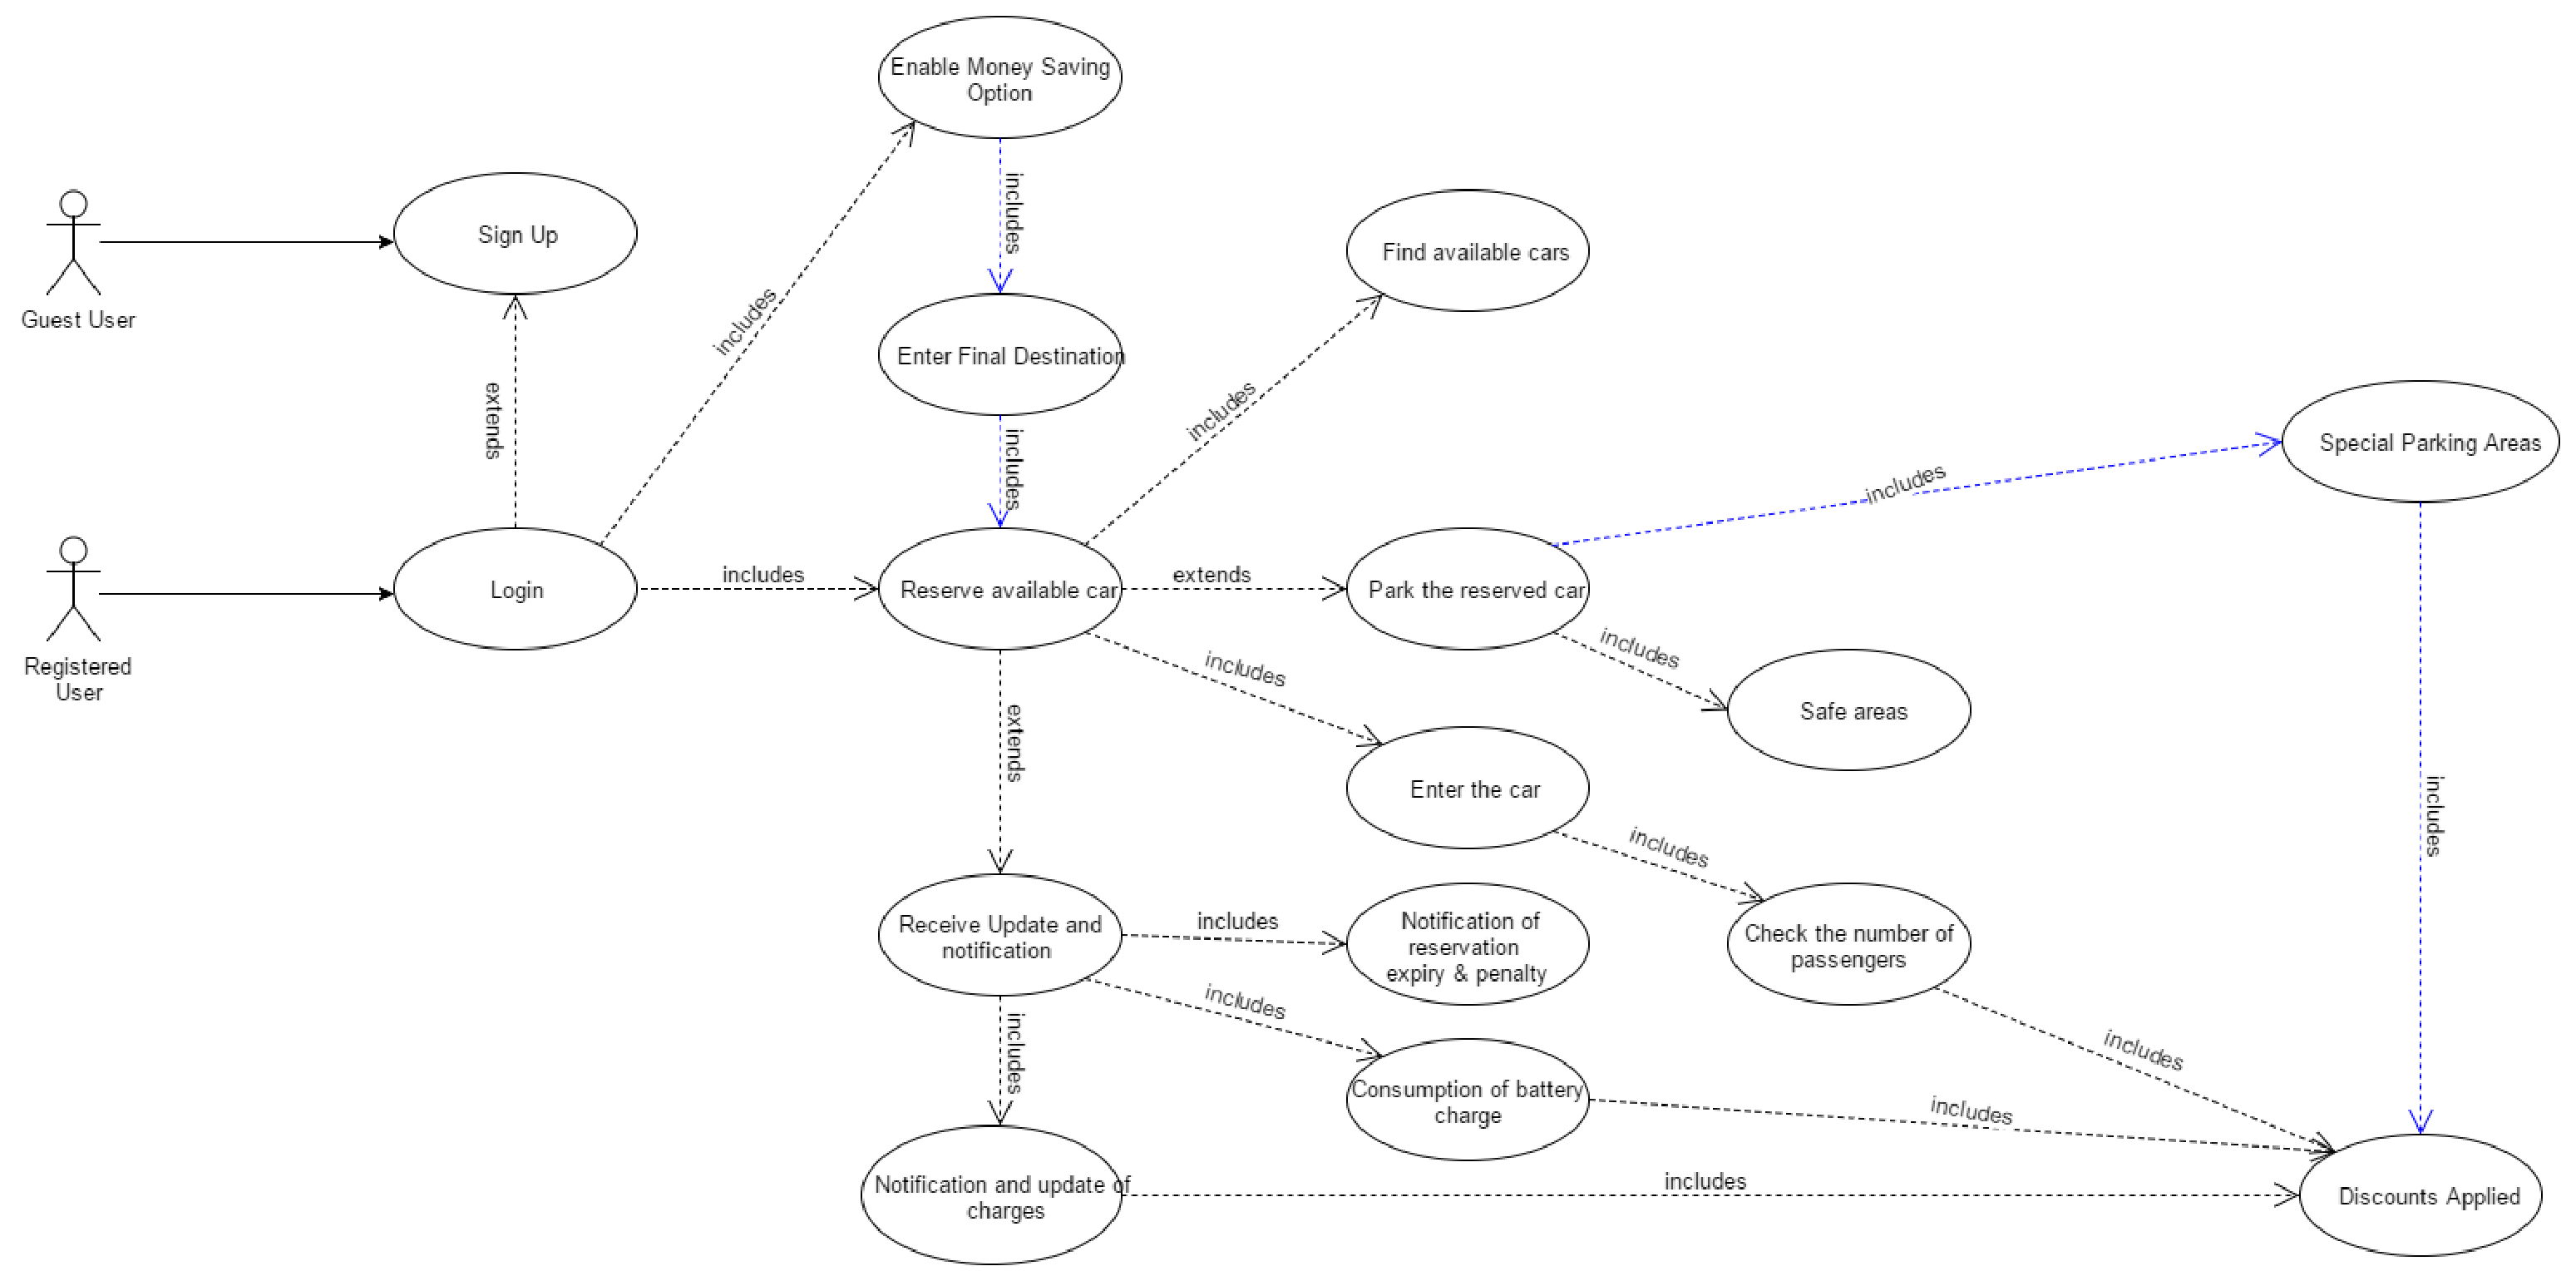
\includegraphics[height=6.7cm,keepaspectratio]{figures/use_case_diagram.eps}
	\caption{Use case diagram for PowerEnJoy}
	\label{fig:use_case_diagram}
\end{figure}

\subsection{Guest sign-up}
\begin{itemize}
	\item \emph{Actors}: Unregistered user
	\item \emph{Entry conditions}: User must not be registered.
	\item \emph{Flow of events}:
	\begin{itemize}
		\item The user arrives at the home page of the mobile app or desktop version.
		\item The user clicks on the Sign Up button.
		\item The user inputs its personal data, including one valid ID and a valid drive license.
		\item The user must confirm the registration browsing a link sent by the system to the email address specified by the user.
		\item The system checks the profile and the input data are validated.
		\item The user must input in the app's homepage the 6 digit code sent by the system to the specified mobile number.
		\item The system validates the account, the user gets notified by sms and notification.
	\end{itemize}
	\item \emph{Exit conditions}: User's account is validated.
	\item \emph{Exceptions}: If the system rejects the input data, the user can find explanations in the app's home page, where he can insert the missing data. If the user doesn't receive the SMS he can ask the app to send it again.
\end{itemize}

\subsection{User login}
\begin{itemize}
	\item \emph{Actors}: Registered user
	\item \emph{Entry conditions}: User must have a confirmed account.
	\item \emph{Flow of events}:
	\begin{itemize}
		\item The user arrives at the homepage of the mobile app or desktop version.
		\item The user inputs its credentials in the drop-down menu.
		\item The user clicks on login.
		\item The user is redirected to his personal page.
	\end{itemize}
	\item \emph{Exit conditions}: The user is successfully redirected to his personal page.
	\item \emph{Exceptions}: The credentials specified by the user were wrong. The user is notified and he can input them again.
\end{itemize}

\subsection{User reserves an available car}
\begin{itemize}
	\item \emph{Actors}: Registered user
	\item \emph{Entry conditions}: User must have a validated account and be logged in.
	\item \emph{Flow of events}:
	\begin{itemize}
		\item The user arrives at his personal page of the mobile app or desktop version.
		\item The user clicks on Find Available Car to full size the map.
		\item The user selects a car and clicks Reserve.
		\item The user is notified with both SMS and app notification about the reservation and the instructions to abort it.
		\item The user approaches the car.
		\item The user asks the system to unlock the car.
		\item The system checks the user's position through the GPS.
		\item If the user's GPS position matches with the car's one, the car is unlocked.
		\item The user can specify whether to enable the Money Saving Option and the destination (mandatory if this option is enabled).
		\item The user ignites the engine and the system starts charging.
		\item The system takes notes about the number of passengers.
		\item The user drive to his destination.
		\item If the Money Saving Option is enabled, the system suggests the user the special parking area where to park.
		\item The user looks for an available parking spot, while verifying on the app's map that it's not forbidden by the service's policies.
		\item The user parks the car.
		\item The user stops the engine and the system stops charging.
		\item The user leaves the car.
		\item If the parking area isn't forbidden the car gets locked by the system, otherwise the user will be asked to get back in the car and change parking spot.
		\item The system checks the battery status, the distance between the parking slot and the closest power station grid, and along with the previously acquired number of passengers, it applies penalties and discount according to the terms and conditions.
		\item The user gets notified about the final charge along with the discounts.
	\end{itemize}
	\item \emph{Exit conditions}: The user gets notified by the system and the car is locked.
	\item \emph{Exceptions}: If the GPS positions of the car and the user don't match, the user is notified to get closer to the car. If the user parks in a low GPS coverage area, the system will notify the user in time. The same if the user parks in a non-safe area. If the user doesn't get back in the car within X minutes, the car gets locked and the user gets penalties.
\end{itemize}

\newpage
\section{Sequence diagrams}

\subsection{Registration of a user}
\begin{figure}[h]
	\centering
	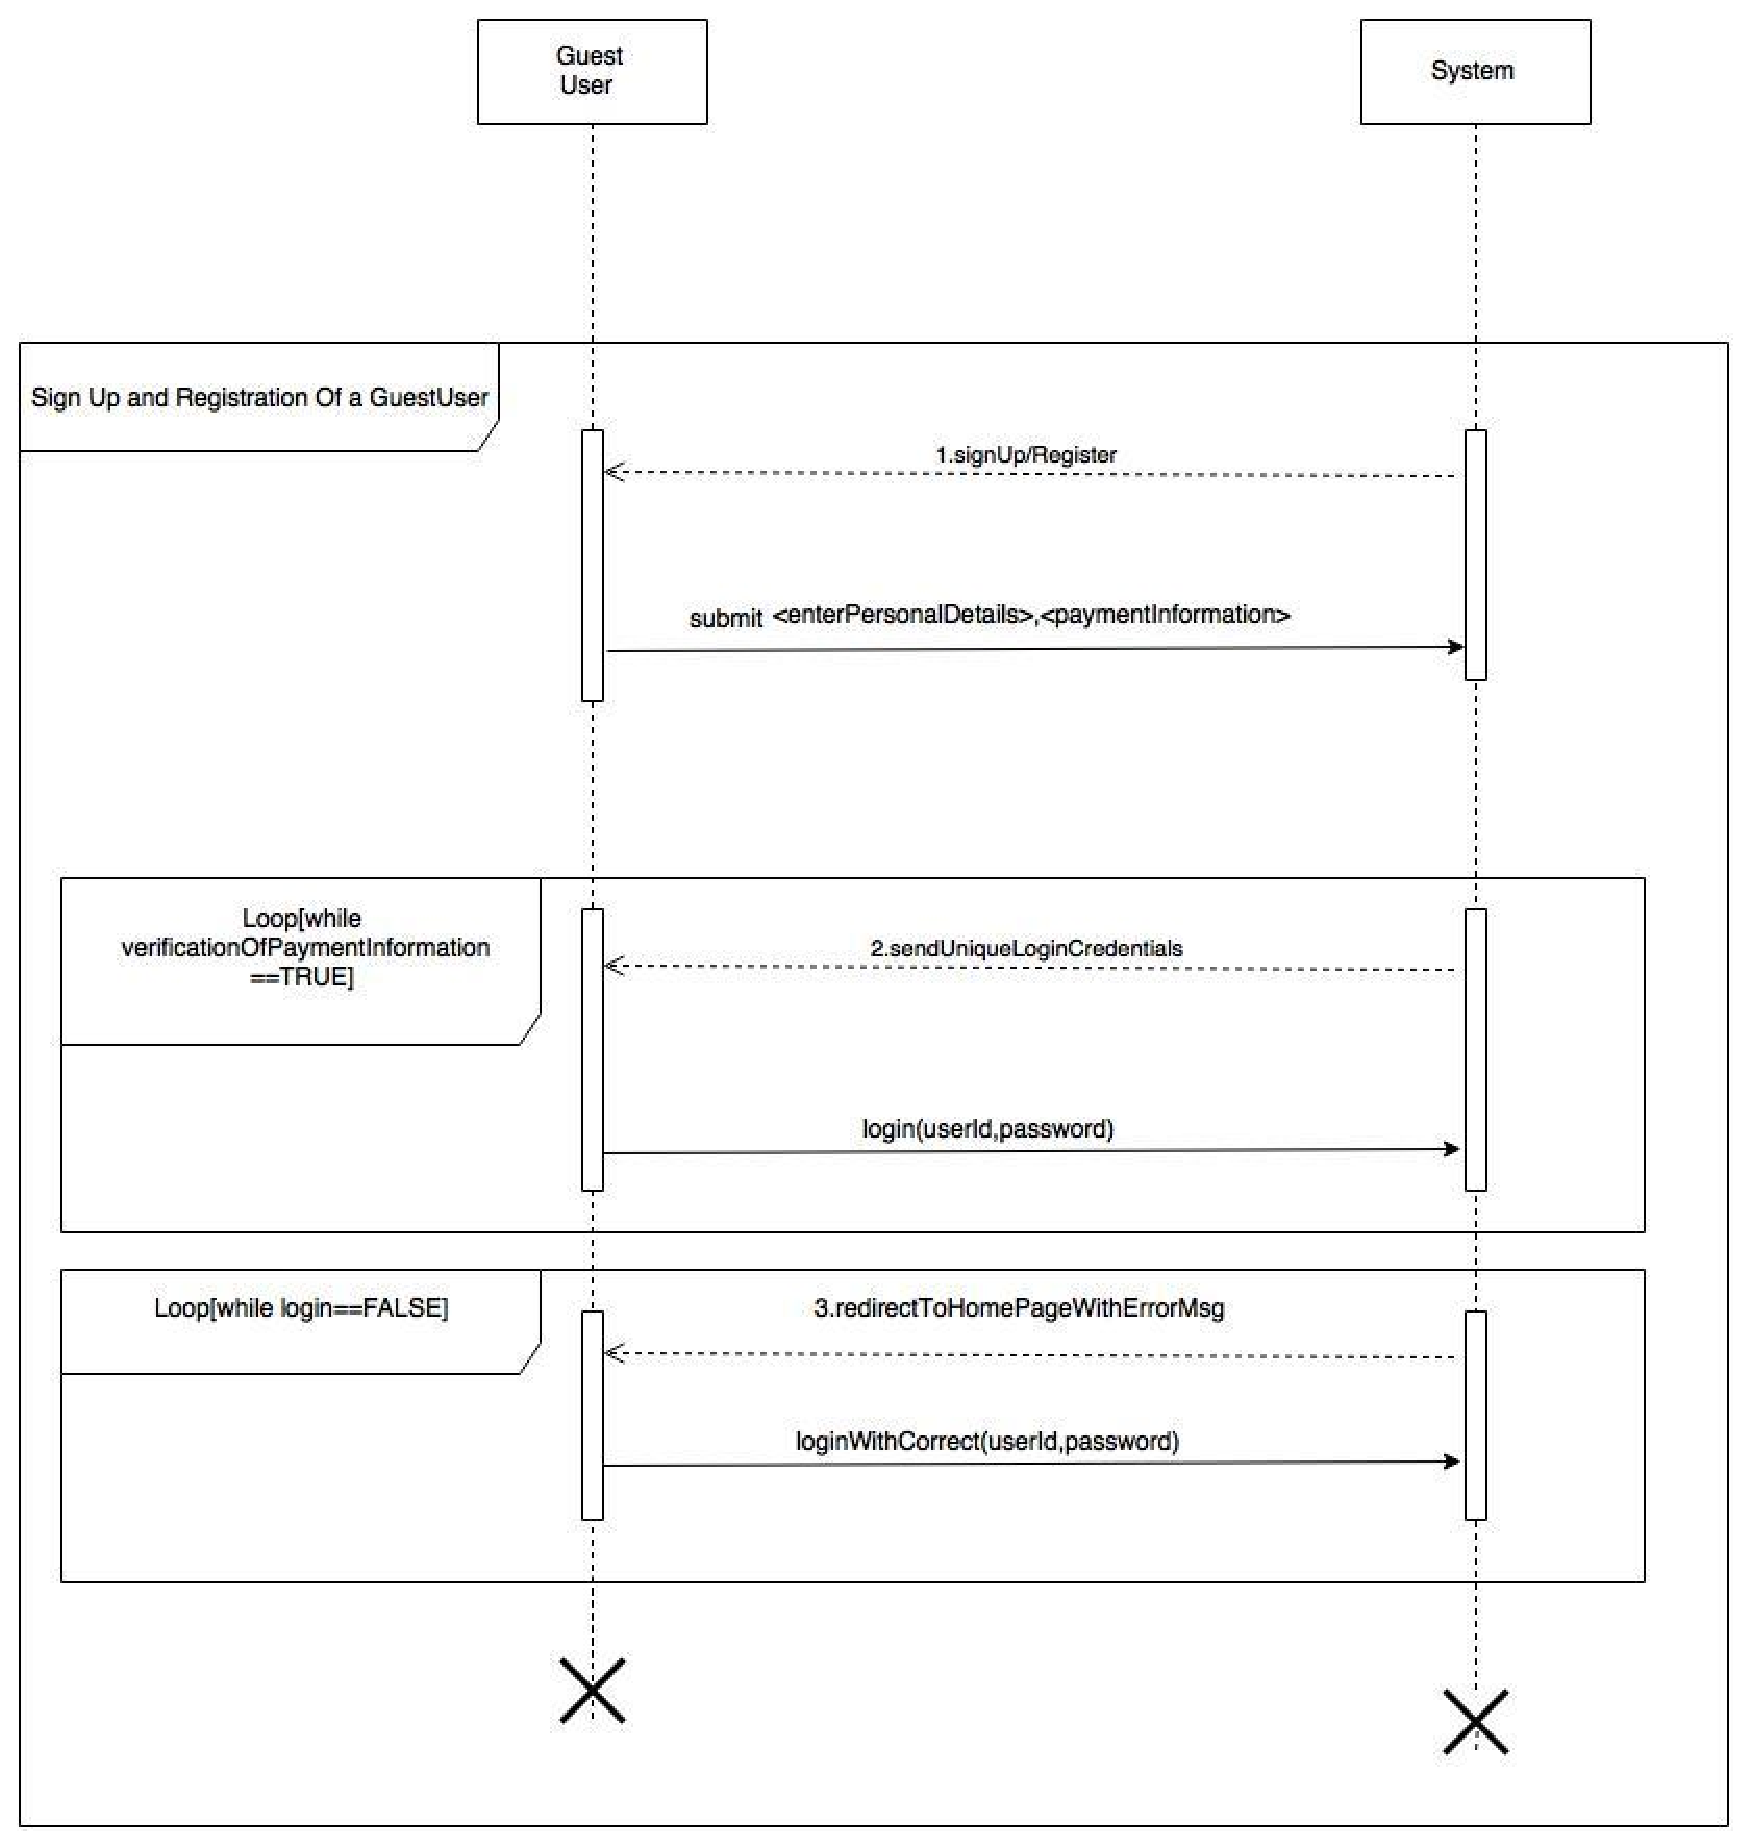
\includegraphics[height=15.2cm,keepaspectratio]{figures/sequence_register.eps}
	\caption{Sequence diagram for the registration of a user}
	\label{fig:sequence_register}
\end{figure}

\newpage
\subsection{Reservation of a car}
\begin{figure}[h]
\centering
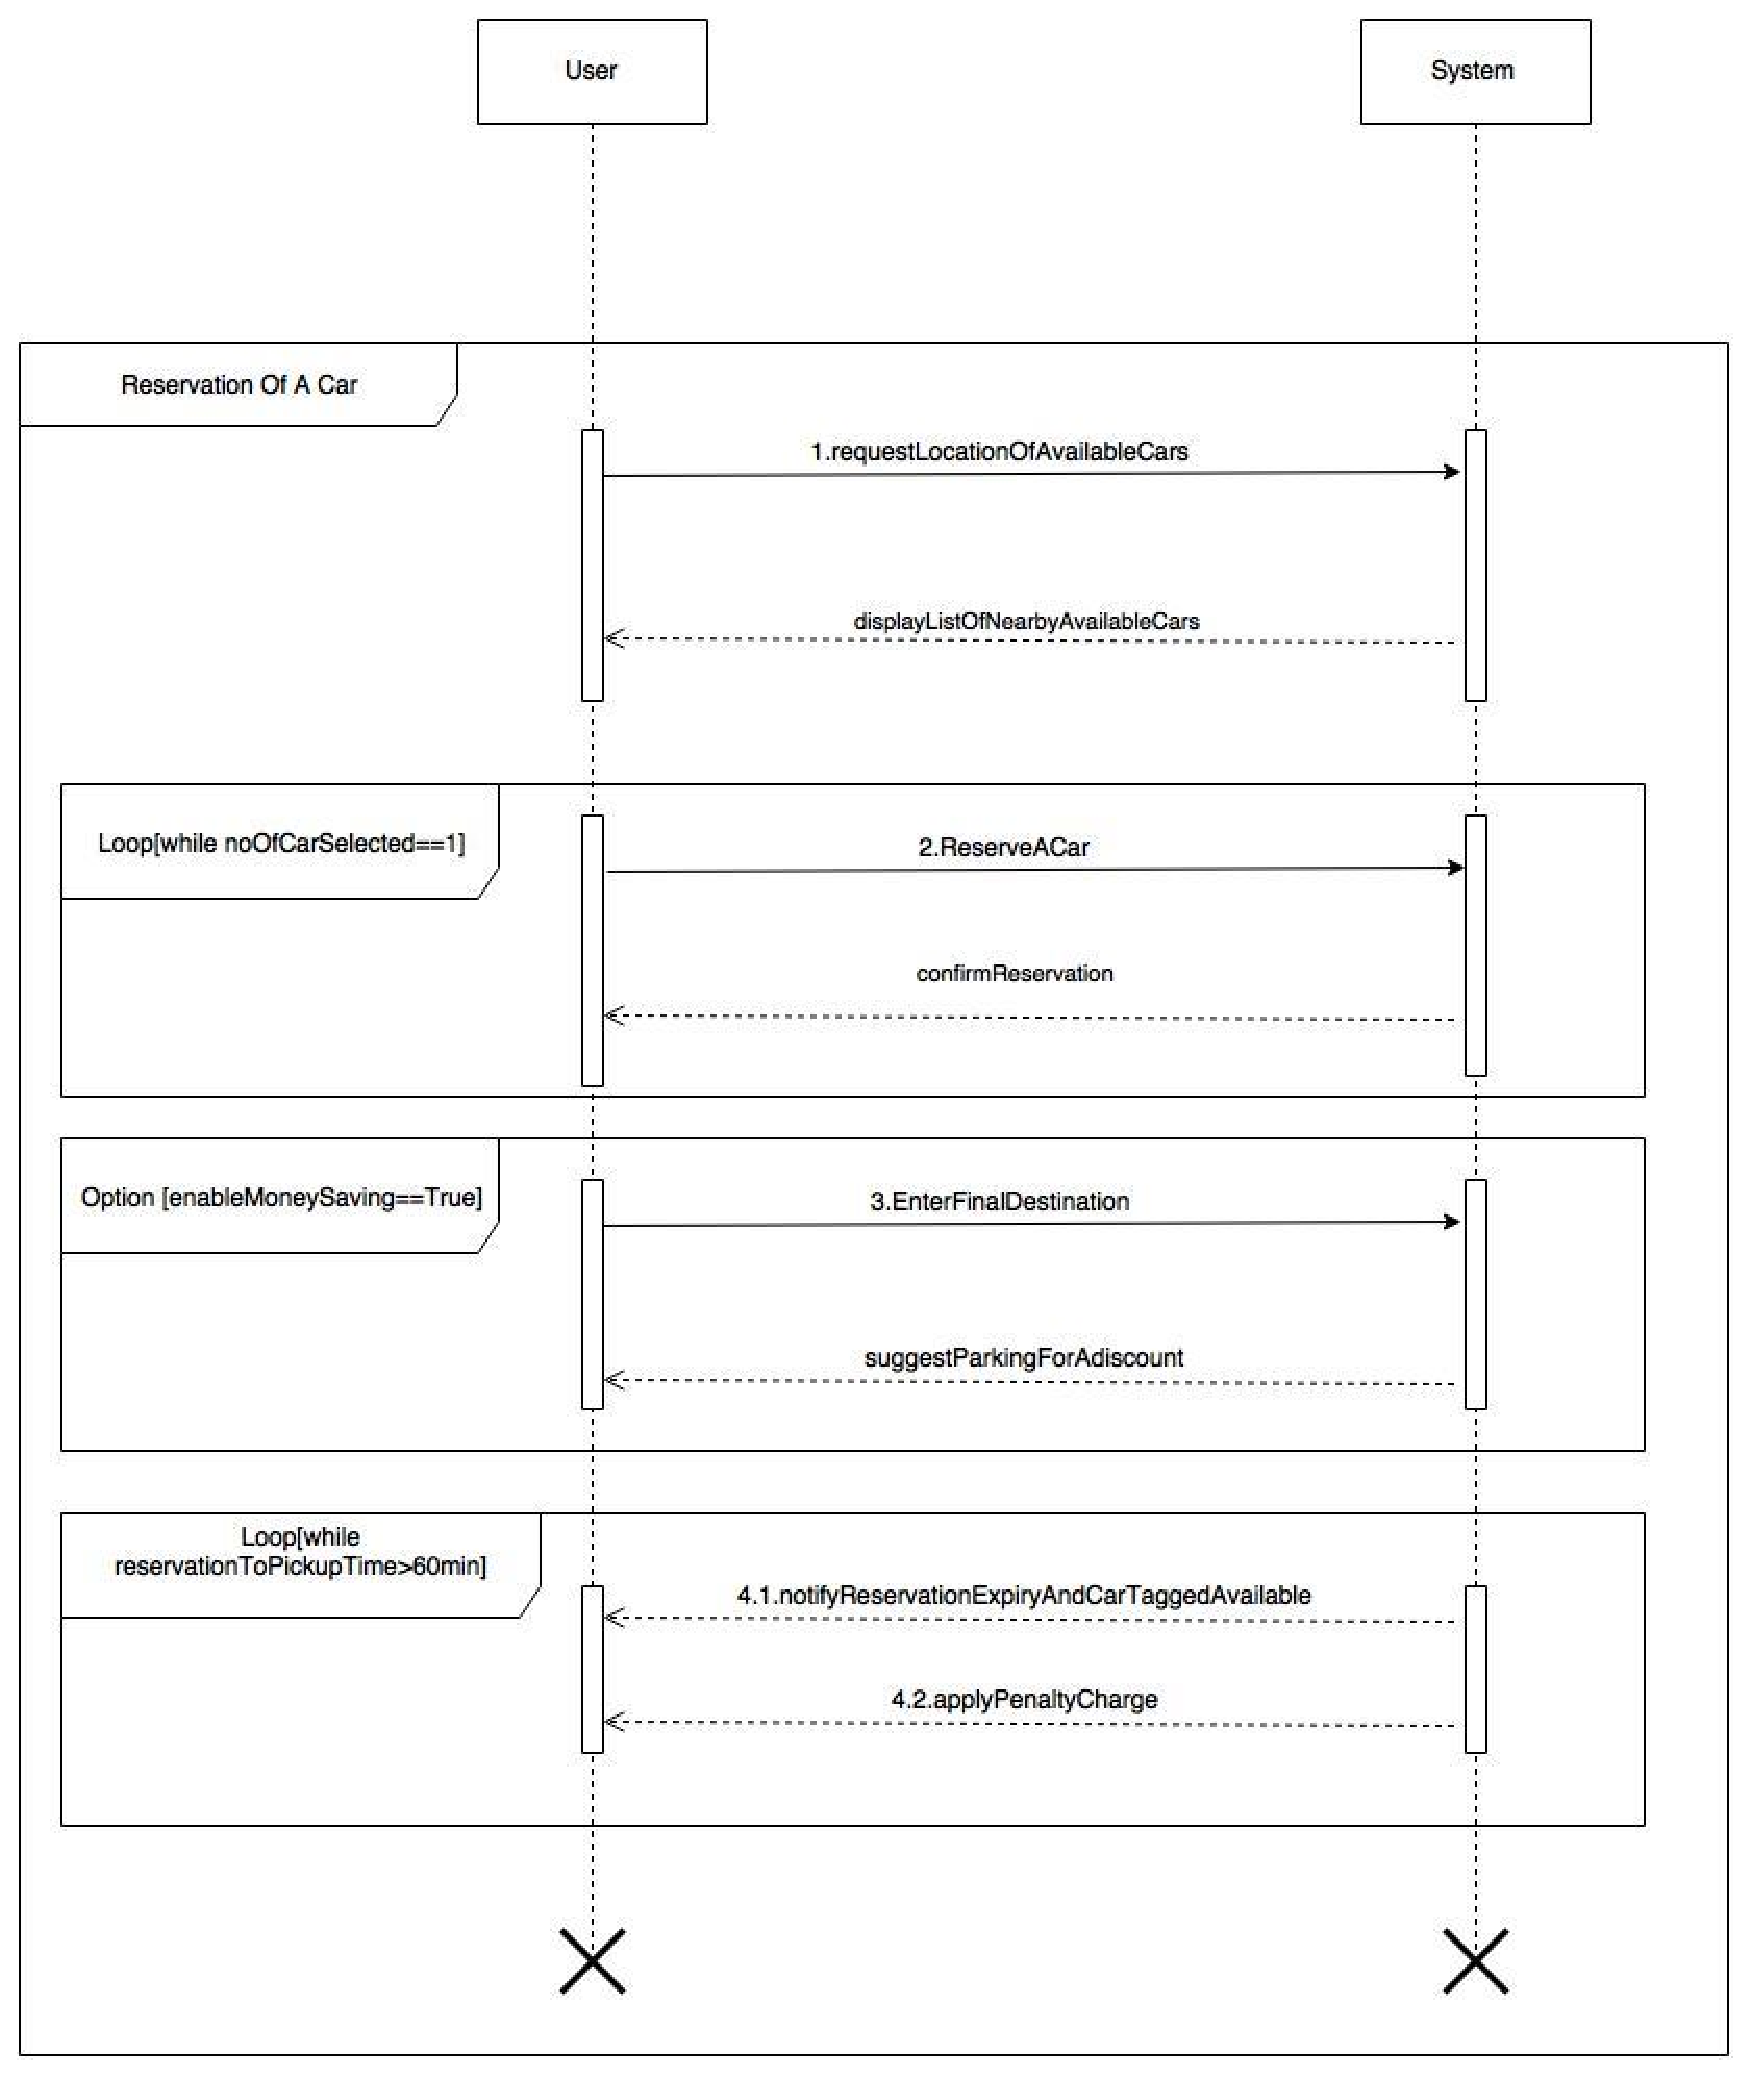
\includegraphics[height=15.2cm,keepaspectratio]{figures/sequence_reservation.eps}
\caption{Sequence diagram for the reservation of a car}
\label{fig:sequence_reservation}
\end{figure}

\newpage
\subsection{Discounts}
\begin{figure}[h]
\centering
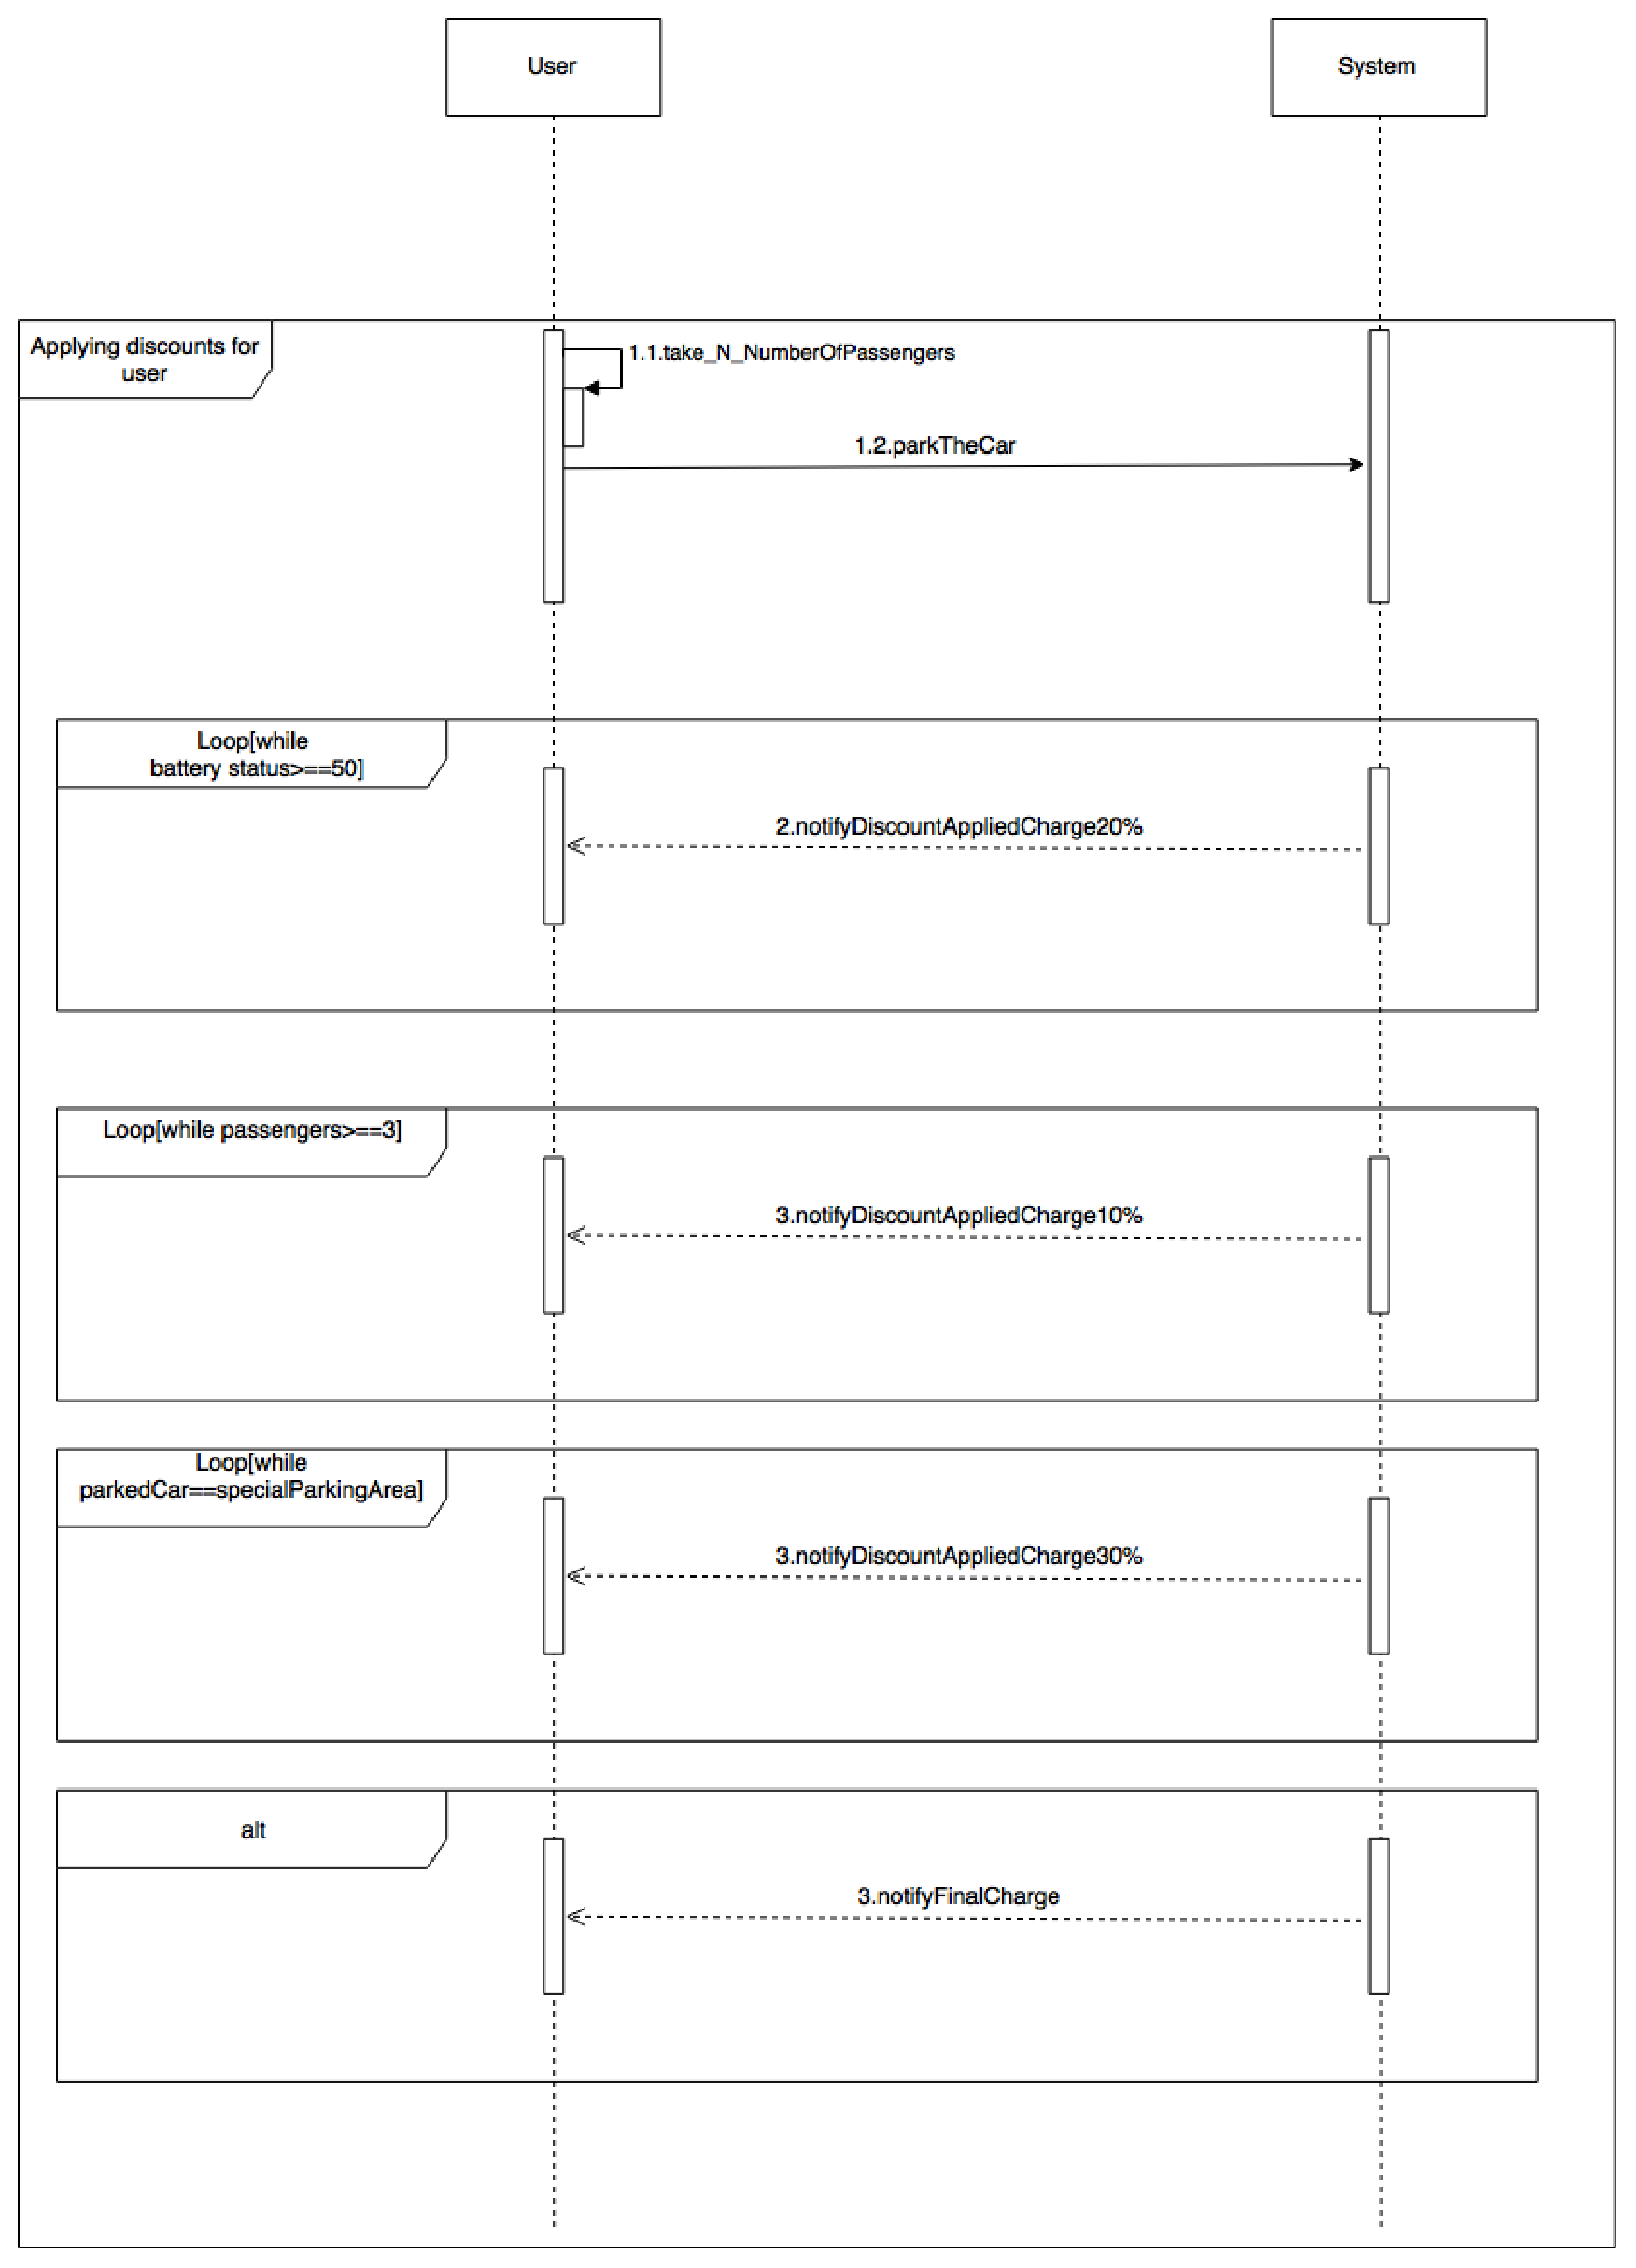
\includegraphics[height=15.2cm,keepaspectratio]{figures/sequence_discounts.eps}
\caption{Sequence diagram for the application of discounts}
\label{fig:sequence_discounts}
\end{figure}

\newpage
\section{Class diagram}
\begin{figure}[h]
	\centering
	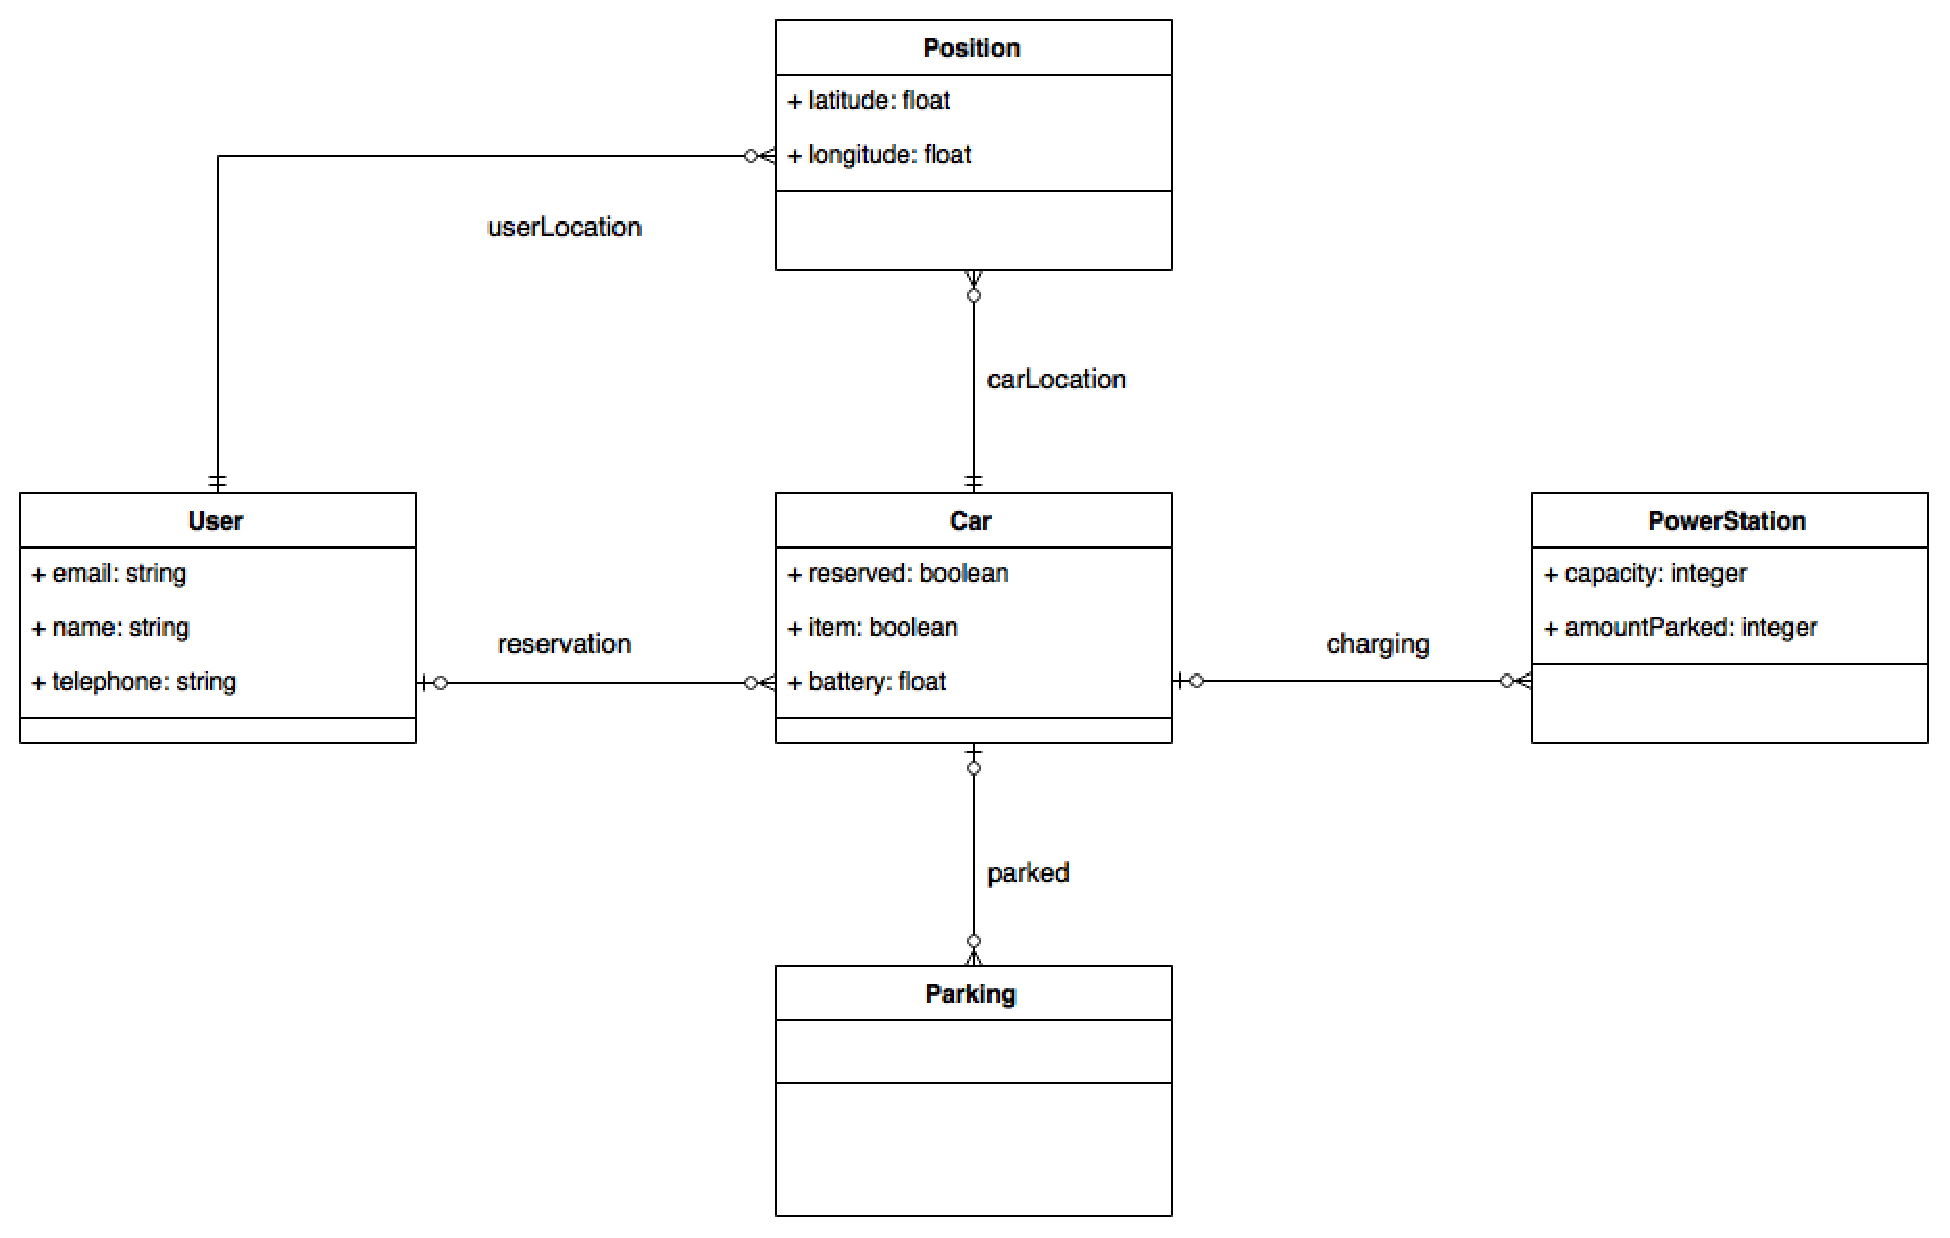
\includegraphics[width=\textwidth,keepaspectratio]{figures/class_diagram.eps}
	\caption{Class diagram for PowerEnJoy}
	\label{fig:class_diagram}
\end{figure}

\newpage
\section{Activity diagrams}

\begin{figure}[h]
	\centering
	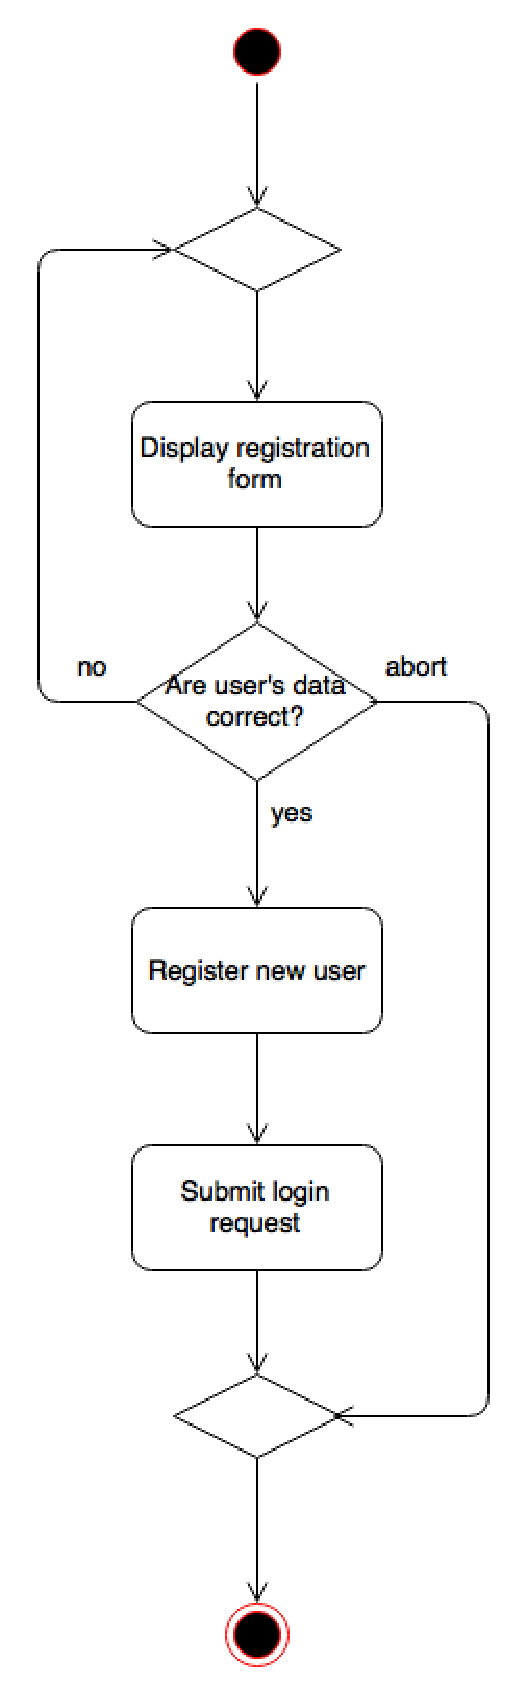
\includegraphics[height=15.2cm,keepaspectratio]{figures/registration_activity_diagram.eps}
	\caption{Activity diagram for the registration of a user}
	\label{fig:registration_activity_diagram}
\end{figure}

\newpage
\begin{figure}[h]
	\centering
	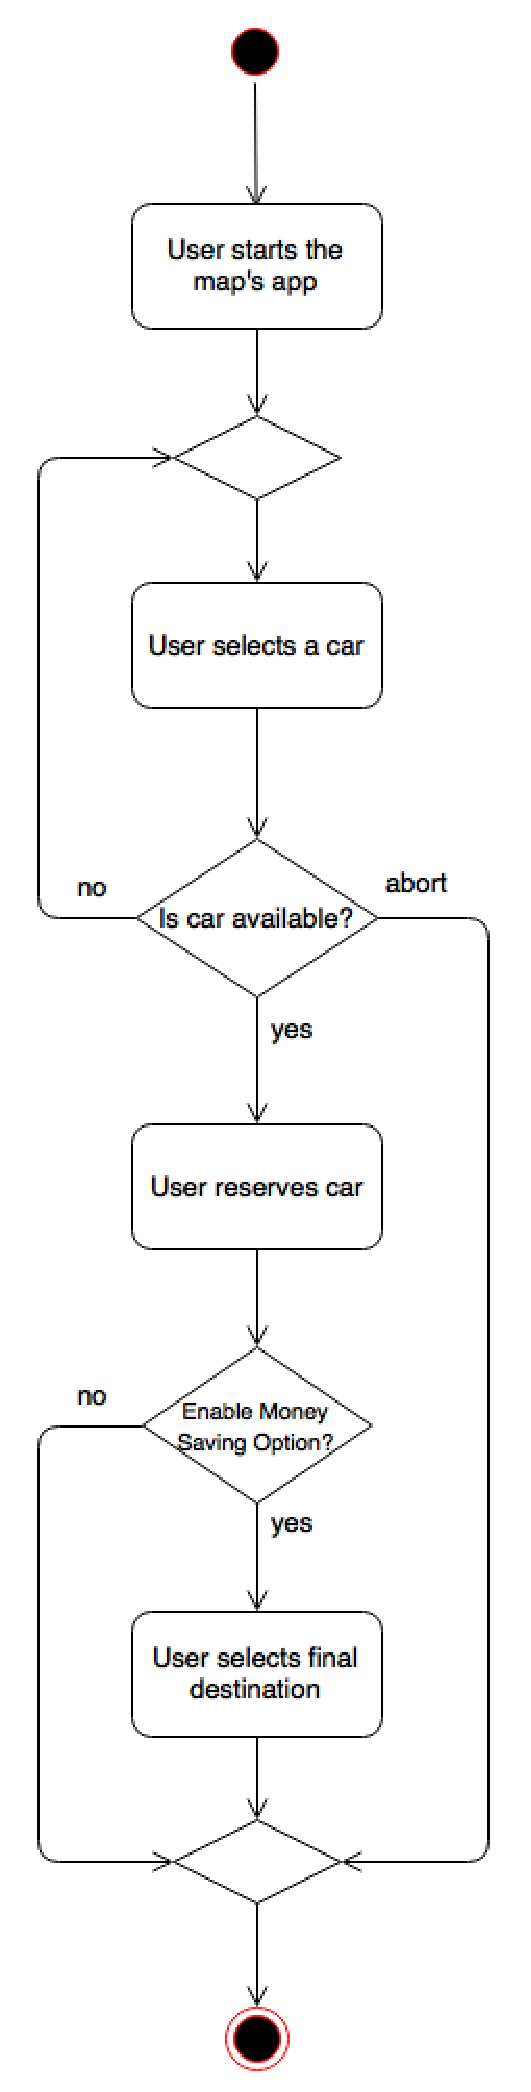
\includegraphics[height=20cm,keepaspectratio]{figures/reservation_activity_diagram.eps}
	\caption{Activity diagram for the reservation of a car}
	\label{fig:reservation_activity_diagram}
\end{figure}
\chapter{Hours of work}

\section{Francesco Fabiani}
\begin{itemize}
	\item 23/10/2016: 1h30min
	\item 24/10/2016: 2h
	\item 25/10/2016: 1h
	\item 26/10/2016: 1h
	\item 27/10/2016: 1h
	\item 29/10/2016: 2h
	\item 02/11/2016: 3h
	\item 03/11/2016: 1h30min
	\item 05/11/2016: 2h
	\item 07/11/2016: 1h
	\item 08/11/2016: 2h30min
	\item 10/11/2016: 2h
	\item 11/11/2016: 3h
	\item 12/11/2016: 2h30min
	\item 13/11/2016: 4h
\end{itemize}

\section{Jagadesh Manivannan}
\begin{itemize}
	\item 22/10/2016: 1h
	\item 23/10/2016: 1h
	\item 25/10/2016: 1h30min
	\item 26/10/2016: 1h
	\item 27/10/2016: 2h
	\item 29/10/2016: 1h
	\item 30/10/2016: 2h30min
	\item 31/10/2016: 1h
	\item 02/11/2016: 2h30min
	\item 03/11/2016: 1h
	\item 04/11/2016: 2h
	\item 06/11/2016: 1h
	\item 07/11/2016: 2h
	\item 08/11/2016: 1h
	\item 09/11/2016: 2h
	\item 10/11/2016: 2h
	\item 11/11/2016: 1h30min
	\item 12/11/2016: 3h
	\item 13/11/2016: 2h30min
\end{itemize}

\section{Niccolò Pozzolini}
\begin{itemize}
	\item 24/10/2016: 2h
	\item 25/10/2016: 1h
	\item 26/10/2016: 2h
	\item 27/10/2016: 1h
	\item 28/10/2016: 1h30min
	\item 29/10/2016: 2h
	\item 01/11/2016: 2h
	\item 02/11/2016: 3h
	\item 05/11/2016: 1h
	\item 06/11/2016: 1h
	\item 08/11/2016: 3h
	\item 10/11/2016: 2h
	\item 11/11/2016: 1h30min
	\item 12/11/2016: 3h30min
	\item 13/11/2016: 4h
\end{itemize}

\end{document}